\myChapter{Testy}\label{ch:tests}
%************************************************

\section{Cele}

Głównym zadaniem przeprowadzonych testów było zbadanie zachowania stworzonego systemu i oprogramowania pod kątem wykorzystania w grach wideo\graffito{Wynika to ze studiowania na specjalności Technologii Gier i Symulacji Komputerowych}. Nie jest jednak trudno sobie wyobrazić inne dziedziny, w których można wykorzystać systemu, jak np.:
\begin{itemize}
 \item medycyna \ppauza manipulacja trójwymiarowymi obrazami skanów pacjentów,
 \item cyfrowe modelarstwo \ppauza szybkie prototypowanie modeli,
 \item tworzenie filmów \ppauza przechwytywanie ruchu.
\end{itemize}

Głównym atutem systemu w tych polach jest naturalny sposób manipulacji i~interakcji z komputerem ze względu na pobieranie dodatkowo \ppauza w odróżnieniu od standardowego zostawu klawiatura + myszka \ppauza trzeciego wymiaru.

\section{Metody}
Aby określić przydatność systemu, należy zbadać kilka czynników. Ich wagi będą różnić się, w zależności od planowanego wykorzystania, jednak można zauważyć, że należy dążyć do optymalizacji cech takich jak:
\begin{itemize}
 \item dokładność,
 \item stabilność,
 \item niezawodność,
 \item prostota użytkowania,
 \item kompatybliność z oprogramowaniem,
 \item szybkość.
\end{itemize}


\section{Wyniki}
% dokladnosc
Dokładność systemu została już określona w sekcji \ref{section:precision}, pozwolę więc sobie jedynie przytoczyć obliczone parametry.

Istnieją dwa rodzaje ograniczeń: spowodowane stworzonym oprogramowaniem oraz spowodowane wykorzystanym sprzętem. Ominięcie tych pierwszych jest stosunkowo łatwe\graffito{Trzeba liczyć się z faktem, że można natknąć się na ograniczenia mikrokontrolera} i~wymaga tylko zmiany pewnych parametrów oraz ponowne zaprogramowanie układu. W przypadku drugiego typu ograniczeń należy spodziewać się konieczności modyfikacji układu, jeśli chciałoby się zwiększać dokładność.

Mikrokontroler jest w stanie mierzyć pozycję markera z dokładnością do 0.34mm\graffito{Równania odpowiednio \ref{eq:microcontroller_limit} i \ref{eq:sound_limit}}, natomiast wykorzystanie sygnałów ultradźwiękowych o częstotliowści 40kHz nakłada na system ograniczenie dokładności do 8.5mm, a zatem ograniczenie całego systemu wynosi 8.5mm.

Chociaż w wielu przypadkach taka dokładność jest zupełnie wystarczająca, pozostawia jednak trochę do życzenia.

% stabilnosc
Pomimo przytoczonej powyżej, relatywnie małej, dokładności układ wykazuje pewną niestabilność, która objawia się drganiem odtworzonej pozycji markera. Widać to dobrze na rysunku \ref{fig:charter_shaky}, którego górna część pokazuje odtworzoną pozycję w trzech wymiarach. Wszystkie dane, a w szczególności wartość $Y$, wykazują kilkucentymetrowe drgania pomimo stabilnego umocowania zarówno układu jak i markera.

\begin{figure}
 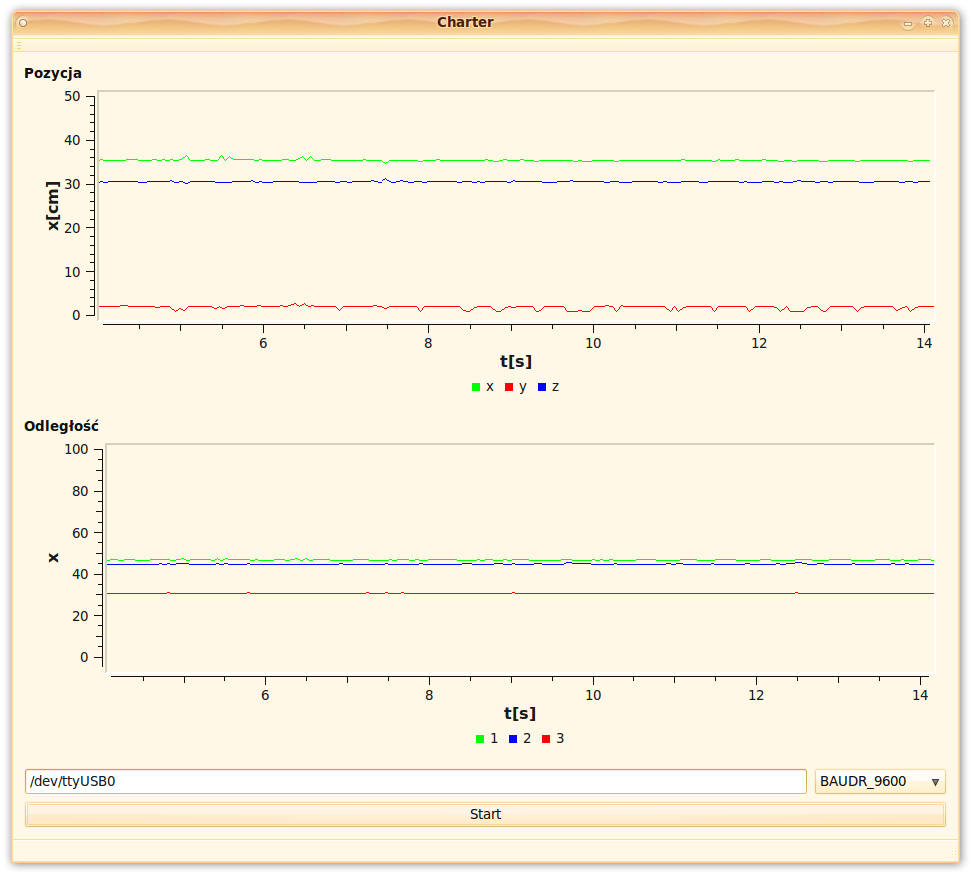
\includegraphics[width=\textwidth]{gfx/charter_shaky.png}
 \caption[Wykres pozycji i odległości jednego z markerów]{Wykres pozycji i odległości od czujników jednego z~markerów w~stałej pozycji}
 \label{fig:charter_shaky}
\end{figure}

% niezawodność
\graffito{coś trzeba napisać o niezawodności}

% kompatybilność z oprogramowaniem
Program wykorzystuje do komunikacji z komputerem protokół \textsmaller{RS232}. Jest to standard komunikacji szeregowej niegdyś bardzo często dostępny w komputerach, jednak dziś odpowiednie złącza i interfejsy dostępne są za sprawą stosunkowo niedrogich adapterów wpinanych do portu \textsmaller{USB}.

Chociaż do uruchomienia komunikacji z wykorzystaniem modułu \textsmaller{USART}\graffito{\textsmaller{USART} \ppauza Universal Synchronous and Asynchronous serial Receiver and Transmitter} mikrokontrolera nie jest wymagane stosowanie zewnętrznego oscylatora, to jego wykorzystanie zmniejsza ilość błędów, jakie mogą zachodzić podczas transmisji.

Ze względu na brak możliwości zakupu stosownego oscylatora, zdecydowałem się wykorzystać wbudowany w mikrokontroler zadajnik częstotliowści. W takiej konfiguracji, w przypadku transmisji danych z prędkością 9600bps\graffito{bps \ppauza baud per second} błąd wynosi zaledwie 0.2\%.

Moje doświadczenie z mikrokontrolerami pokazuje, że wartość ta jest dostatecznie mała, aby można było założyć, że trasmisja jest dokładna.

Wykorzystany do komunikacji interfejs oraz zaproponowany protokół\graffito{opisać protokół} jest bardzo prosty, co pozwala na dodanie obsługi systemu do dowolnego programu pragnącego skorzystać z tej możliwości znikomym nakładem pracy.

Stanowiłoby to duży atut systemu w przypadku jego popularyzacji.